\documentclass[11pt]{article}
\usepackage{icmlko}
\begin{document}

\title{절반은 아무것도 아니다 --- 만화가 누르는 것은 양이 아니라 있음이다}
\author{월드모델 실험실}
\date{노트 361 · 2026년 8월 1일}
\maketitle

\begin{abstract}
노트 356이 채점 안 되는 도메인 하나를 찾았다 --- 만화는 학습 1,783행
(전체의 17\%)인데 유보 6행이라 \texttt{evaluate} 문턱 20을 못 넘어 한 번도
채점되지 않는다. 빼면 판이 오른다. 왜인지는 못 밝혔고 라벨 종류로도 안
갈렸다. \textbf{이분법으로 갈랐다.} 미리 적었다: 희석이면 절반을 빼면
절반이 나와야 한다. \textbf{안 나왔다} --- 절반(892행) 빼기가 판
$-0.0008$(SD 0.0046, \textbf{6/12})로 정확히 0 이고, 전부(1,783행) 빼기가
$+0.0041$(SD 0.0062, 8/12)이다. \textbf{희석이 아니다.} 만화가 무는 값은
행 수를 안 따른다 --- 절반이 남아 있으면 전부 남아 있는 것과 같다.
도메인별로 보면 예외가 하나 있다: \textbf{아이돌만 양을 따른다}
($+0.0342 \to +0.0587$). 나머지 아홉은 절반에서 아무 일도 안 난다.
그리고 노트 356의 $+0.0058$ 은 지금 판에서 $+0.0041$ 이다 --- 그 사이에
챔피언이 두 번 바뀌었으므로 옛 수를 그대로 쓰면 안 된다는 확인이기도 하다.
\end{abstract}

\section{미리 적은 것}

\begin{quote}
\textbf{희석이면 선형이다} --- C$-$A 가 B$-$A 의 절반($+0.003$ 근처)이어야
한다. \textbf{구조면 포화한다} --- C$-$A 가 B$-$A 에 가깝거나 0 에 가깝다.
\end{quote}

\begin{center}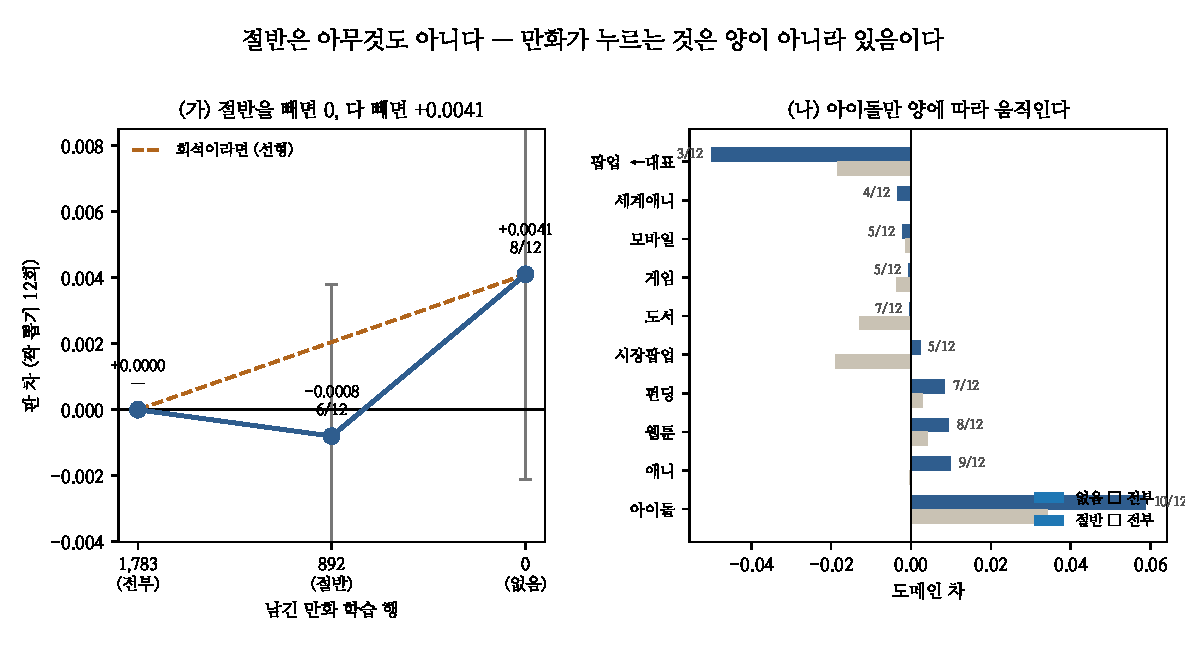
\includegraphics[width=\linewidth]{figs/presence.pdf}\end{center}

\begin{center}
\begin{tabular}{lrrr}
\hline
 & 판 차 & SD & 부호 \\
\hline
절반 남김(892행) $-$ 전부 & $-0.0008$ & 0.0046 & 6/12 \\
없음 $-$ 전부             & $\mathbf{+0.0041}$ & 0.0062 & 8/12 \\
\hline
\end{tabular}
\end{center}

\textbf{희석이 반증됐다.} 예측이 $+0.003$ 이었고 측정이 $-0.0008$ 에
6/12 --- 부호조차 안 선다. 만화 892행을 버리는 것은 아무 일도 아니다.

\section{도메인별로 하나만 다르다}

\begin{center}
\begin{tabular}{lrrrr}
\hline
도메인 & 절반 $-$ 전부 & 부호 & 없음 $-$ 전부 & 부호 \\
\hline
\textbf{아이돌} & $\mathbf{+0.0342}$ & 8/12 & $\mathbf{+0.0587}$ & 10/12 \\
애니     & $-0.0004$ & 6/12 & $+0.0099$ & 9/12 \\
웹툰     & $+0.0041$ & 7/12 & $+0.0094$ & 8/12 \\
펀딩     & $+0.0029$ & 7/12 & $+0.0085$ & 7/12 \\
시장팝업 & $-0.0189$ & 2/12 & $+0.0023$ & 5/12 \\
도서     & $-0.0128$ & 4/12 & $-0.0004$ & 7/12 \\
모바일   & $-0.0015$ & 5/12 & $-0.0021$ & 5/12 \\
게임     & $-0.0036$ & 7/12 & $-0.0006$ & 5/12 \\
세계애니 & $+0.0002$ & 6/12 & $-0.0033$ & 4/12 \\
\textbf{팝업}(대표) & $-0.0185$ & 3/12 & $-0.0500$ & 3/12 \\
\hline
\end{tabular}
\end{center}

\textbf{아이돌만 양을 따른다} --- 절반에서 $+0.0342$, 전부에서 $+0.0587$
로 거의 선형이고 부호도 8/12 · 10/12 로 선다. 아이돌은 유보 51행 ·
학습 122행짜리 얇은 도메인이고, 만화 1,783행이 공유 적합에서 가장
직접적으로 밀어내는 상대인 것으로 보인다.

나머지 아홉은 절반에서 아무것도 안 난다. \textbf{판이 절반에서 0 인 것은
아이돌의 $+0.0342$ 가 가중 1.9\% 라 $+0.0006$ 밖에 안 되고, 그것을
팝업 $-0.0185$(2.4\%)와 시장팝업 $-0.0189$(4.6\%)가 지우기 때문이다.}
노트 351의 환율이 그대로 작동한다.

\section{그래서 무엇이 남았나}

희석을 지웠다. 남은 후보는 셋이다.

\begin{itemize}
\item \textbf{원핫 열} --- F18은 도메인마다 지시 열을 하나 붙인다. 만화를
빼면 열도 사라지고, 절반은 열을 남긴다. 이것이면 고침이 열 하나로 끝난다.
\item \textbf{라벨 순위 섞임} --- F18은 도메인 안에서 $y$ 를 순위로 바꿔
쌓는다. 절반이면 만화 몫이 반이 되므로 이것이라면 부분 효과가 났어야
한다. \emph{안 났으니 약하다.}
\item \textbf{자리 차지} --- 만화 행이 공유 특징 공간의 어떤 자리를
채우고 공유 적합을 그리로 당긴다. 밀도를 반으로 줄여도 자리는 그대로다.
\end{itemize}

두 번째는 이 실험이 이미 약화시켰다. 첫째와 셋째를 가르는 것이 다음
노트다 --- 만화를 10\%(178행)만 남기는 팔과, \emph{행은 두고 원핫 열만
빼는} 팔을 붙인다. 10\%가 0 이면 어떤 양이든 있으면 같다는 뜻이고(셋째),
원핫만 빼서 $+0.004$ 가 나오면 범인이 열이다(첫째). 이미 걸어 뒀다.

\section{덧 --- 옛 수를 그대로 쓰면 안 된다}

노트 356이 같은 처치를 $+0.0058$(10/12)로 쟀다. 지금은 $+0.0041$(8/12)이다.
그 사이 챔피언이 두 번 바뀌었다(노트 358의 등급 필터, 노트 353의 아이돌
유보). \textbf{자료 결정의 값은 판이 바뀌면 같이 바뀐다} --- 노트 357이
노트 127$\cdot$132 에서 이미 겪은 것과 같은 자리다($+0.08$ 이 $-0.04$ 가
됐다). \textbf{규약: 남은 것 표의 수는 인용할 때마다 다시 잰다.}

\section{남은 것}

\begin{center}
\begin{tabular}{ll}
\hline
갈래 & 지금 아는 것 \\
\hline
\textbf{원핫이냐 자리냐} & 10\% 팔과 원핫만 빼는 팔. \textbf{돌고 있다} \\
아이돌만 왜 양을 따르나 & 얇은 도메인(학습 122)이 1,783행에 밀리나 \\
팝업 실측 41행 & 노트 360. 수집 \\
만화 2026 스무 건 & 노트 356. 열한 번째 채점 도메인 \\
\hline
\end{tabular}
\end{center}

\end{document}
